\documentclass{beamer}
\usepackage{amsfonts}
\usepackage{amsmath}
\usepackage{times}
\usepackage{mathrsfs}
\usepackage{extarrows}
\usepackage{bbm} 
\setbeamercolor{footcolor}{fg=blue!100} % 设置字体和背景颜色
\setbeamertemplate{headline}{%
  \leavevmode%
  \hbox{%
    \hskip228pt
    \begin{beamercolorbox}[wd=.126\paperwidth,ht=2.25ex,dp=1ex,right]{footcolor}%      
       \textcolor[rgb]{0,0.168,0.376}{Slide \insertframenumber{} }
    \end{beamercolorbox}}%
  \vskip-19pt%
}

\setbeamertemplate{frametitle}
{
\vspace{30pt}\textcolor[rgb]{0,0.168,0.376}{\insertframetitle}
}

 
\pgfdeclareimage[height=0.61cm]{university-logo}{logo.png}  
\logo{\pgfuseimage{university-logo}{\vspace{244pt}}} 
\title{\textcolor[rgb]{0,0.168,0.376}{VV286 RC4}}
\author{JIANG Yicheng}
\begin{document}

\begin{frame}
\titlepage
\end{frame}


\begin{frame}
\frametitle{Complex Analysis}
We say that a function $f : \mathbb{C}\rightarrow\mathbb{C}$ is complex
differentiable, or holomorphic, at $z \in\mathbb{C}$ if
$$f'(z):=\lim_{h\rightarrow0\atop h\in\mathbb{C}}\dfrac{f(z+h)-f(z)}{h}$$
exists.
\begin{block}{}
We say that a function is holomorphic on an open set $\Omega\subset \mathbb{C}$ if it is holomorphic at every $z \in \Omega$. A function that is holomorphic on $\mathbb{C}$ is called \textcolor[rgb]{0,0.6,0.3}{\textit{\textbf{entire}}}.
\end{block}

\end{frame}

\begin{frame}
\begin{block}{Three Main Properties}
\begin{enumerate}
\item A holomorphic function is automatically infinitely often differentiable (\textcolor[rgb]{0,0.6,0.3}{\textbf{\textit{Cauchy Integral Formulas P331/P334}}})
\item A holomorphic function is automatically analytic (has a power series expansion)(\textcolor[rgb]{0,0.6,0.3}{\textbf{\textit{P337}}});
\item Any closed curve integral of a holomorphic function is vanishes.(\textcolor[rgb]{0,0.6,0.3}{\textbf{\textit{Cauchy's Theorem}}})
\end{enumerate}
\end{block}

\end{frame}

\begin{frame}
\begin{block}{The Cauchy-Riemann Differential Equations}
For a complex function
$$f:\mathbb{C}\rightarrow\mathbb{C},\hspace{3mm}f(x+iy)=u(x,y)+iv(x,y)$$
where $u,v:\mathbb{R}^2\rightarrow\mathbb{R}$, if $f$ is complex differentiable, then
$$\dfrac{\partial u}{\partial x}=\dfrac{\partial v}{\partial y},\hspace{3mm}\dfrac{\partial u}{\partial y}=-\dfrac{\partial v}{\partial x}$$
Suppose that the partial derivatives of $u$ and $v$ exist, are continuous and satisfy the Cauchy-Riemann equations. Then $f$ is holomorphic.
\end{block}

\end{frame}

\begin{frame}
\begin{block}{}
Define differential operators
$$\dfrac{\partial }{\partial z}=\dfrac{1}{2}\Big(\dfrac{\partial }{\partial x}+\dfrac{1}{i}\dfrac{\partial }{\partial y}\Big),\hspace{3mm}\dfrac{\partial }{\partial \overline{z}}=\dfrac{1}{2}\Big(\dfrac{\partial }{\partial x}-\dfrac{1}{i}\dfrac{\partial }{\partial y}\Big)$$
For holomorphic function,
$$f'(z)=\dfrac{\partial f}{\partial z}=2\dfrac{\partial u}{\partial z},\hspace{3mm} \dfrac{\partial f}{\partial \overline{z}}=0$$

If $f$ is a holomorphic function given by $f(x + iy) = u(x, y) + v(x,y)i$, then $u$ and $v$ are harmonic, i.e.
$$\Delta u=\dfrac{\partial^2u}{\partial x^2}+\dfrac{\partial^2u}{\partial y^2}=0,\Delta v=\dfrac{\partial^2v}{\partial x^2}+\dfrac{\partial^2v}{\partial y^2}=0$$
\end{block}
\end{frame}

\begin{frame}
\begin{block}{Relation to Vector Field}
For a vector field $F:\Omega\rightarrow\mathbb{R}^2$, if it's divergence and rotation are zero, i.e.
$$\exists U:\mathbb{R}^2\rightarrow\mathbb{R},F=\nabla U, \hspace{3mm}\text{i.e.}\hspace{1mm}F_1=\dfrac{\partial U}{\partial x},F_2=\dfrac{\partial U}{\partial y}$$
$$\exists V:\mathbb{R}^2\rightarrow\mathbb{R},\hspace{1mm}F_1=\dfrac{\partial V}{\partial y},F_2=-\dfrac{\partial V}{\partial x}$$
Then for function $G=U(x,y)+iV(x,y)$,
$$\dfrac{\partial U}{\partial x}=\dfrac{\partial V}{\partial y},\hspace{3mm}\dfrac{\partial U}{\partial y}=-\dfrac{\partial V}{\partial x}$$
it's holomorphic.
\end{block}
\end{frame}

\begin{frame}
\begin{block}{Sets in the Complex Plane}
\begin{enumerate}
\item A set $\Omega\subset\mathbb{C} $ is called open if for every $z\in\Omega$ there exists an $\varepsilon>0$ such that $B_{\varepsilon}(z)=\lbrace w\in\mathbb{C}:|w-z|<\varepsilon\rbrace\subset\Omega$. A set is called closed if its complement is open.
\item A set $\Omega\subset\mathbb{C}$ is called bounded if $\Omega\subset B_R(0)$ for some $R>0$.
\item A set $K\subset\mathbb{C}$ is called compact if every sequence in $K$ has a subsequence that converges in $K$. A set $K\in\mathbb{C}$ is compact if and only if it is closed and bounded.
\item An open (closed) set $\Omega\subset\mathbb{C}$ is called disconnected if there exist two open (closed) sets $\Omega_1,\Omega_2\subset\mathbb{C}$ such that $\Omega_1\cap\Omega_2=\emptyset$ and $\Omega=\Omega_1\cup\Omega_2$. If $\Omega$ is not disconnected, $\Omega$ is called connected. A set $\Omega\subset\mathbb{C}$ is conneted if and only if for any two points in $\Omega$ there exists a curve joining them.
\item A \textcolor[rgb]{0,0.6,0.3}{\textit{\textbf{region}}} or \textcolor[rgb]{0,0.6,0.3}{\textit{\textbf{domain}}} in $\mathbb{C}$ is an open and conneted set.
\end{enumerate}
\end{block}
\end{frame}

\begin{frame}
\begin{block}{}
We define the diameter of a set $\Omega\subset\mathbb{C}$ by
$$\text{diam}(\Omega)=\sup_{z,w\in\Omega}|z-w|$$
If $(\Omega_n)$ is a sequence of non-empty compact sets such that $\Omega_{n+1}\subset\Omega_n$ for $n\in\mathbb{N}$ and diam $\Omega_n\rightarrow0$ as $n\rightarrow\infty$, then there exists a unique point $w\in\mathbb{C}$ such that $w\in\Omega_n$ for all $n$.
\end{block}
\end{frame}



\begin{frame}
\begin{block}{Primitive}
Let $\Omega\subset\mathbb{C}$ be an open set, $f:\Omega\rightarrow\mathbb{C}$. A primitive for $f$ is a holomorphic function $F:\Omega\rightarrow\mathbb{C}$ such that $f(z)=F'(z)$ for all $z\in\Omega$.
\end{block}

\begin{block}{}
If a continuous function $f$ has a primitive $F$ in $\Omega$, and $\mathcal{C}^*$ is a curve in $\Omega$ that begins at $w_1$ and ends at $w_2$, then
$$\int_{\mathcal{C}^*}f(z)dz=F(w_2)-F(w_1)$$
Especially, if $\mathcal{C}^*$ is a closed curve, 
$$\int_{\mathcal{C}^*}f(z)dz=0$$
If $f$ is holomorphic in a region $\Omega$ and $f'=0$, then $f$ is constant.
\end{block}
\end{frame}

\begin{frame}
\begin{block}{Integrals along Complex Curves}
Let $\Omega\subset\mathbb{C}$ be an open set, $f$ holomorphic on $\Omega$ and $\mathcal{C}^*\subset\Omega$ an oriented smooth curve. We then define the integral of $f$ along $\mathcal{C}^* $ by 
$$\int_{\mathcal{C}^*}f(z)dz=\int_If(\gamma(t))\cdot\gamma'(t)dt$$
where $\gamma:I\rightarrow \mathcal{C}^* $ is a parametrization of the parameterized curve $\mathcal{C}^*$.
\end{block}
\begin{block}{Curve Length}
$$\ell(\mathcal{C})=\Bigg|\int_{\mathcal{C}}dz\Bigg|$$
$$\int_{-\mathcal{C}^*}f(z)dz=-\int_{\mathcal{C}^*}f(z)dz,\hspace{3mm}\Bigg|\int_{\mathcal{C}^*}f(z)dz\Bigg|\leqslant\ell(\mathcal{C})\cdot\sup_{z\in\mathcal{C}}|f(z)|$$
\end{block}
\end{frame}


\begin{frame}
\frametitle{Cauchy's Theorem}

If $f$ is holomorphic in an open (simple) connected set $\Omega$, and $\mathcal{C}^*$ is a closed curve in $\Omega$,
$$\int_{\mathcal{C}^*}f(z)dz=0$$
\end{frame}

\begin{frame}
\begin{block}{Singularities}
Let $\Omega\subset\mathbb{C}$ be open, $z_0\in\Omega$ and $f:\Omega\setminus\lbrace z_0\rbrace\rightarrow\mathbb{C}$ holomorphic. Then $f$ is said to have a point singularity or isolated singularity at $z_0$.
\begin{enumerate}
\item The singularity is said to be removable if there exists an analytic continuation $\tilde{f}:\Omega\rightarrow\mathbb{C}$. (such $\tilde{f} $ is unique)
\item The singularity is said to be a \textcolor[rgb]{0,0.6,0.3}{\textit{\textbf{pole}}} if $g=1/f$ is holomorphic on $\Omega\setminus\lbrace z_0\rbrace$ and has a removable singularity at $z_0$ such that the analytic continuation $\tilde{g}$ of $g$ satisfies $\tilde{g}(z_0)=0$.
\item The singularity is said to be essential if it is neither removable nor a pole.
\end{enumerate}
\end{block}
\end{frame}


\begin{frame}
\begin{block}{How to judge? }

\end{block}
\begin{block}{Removable Singularity}
Whether $\lim\limits_{z\rightarrow z_0}f$  exists.

e.g. 
$$\lim\limits_{z\rightarrow0}\dfrac{\sin z}{z}=1$$
So $f(z)=\dfrac{\sin z}{z}$ has removable singularity at $z=0$.
\end{block}
\begin{block}{Pole (Informal way)}
$f(z)=\dfrac{g(z)}{h(z)}$, then all $z_0$ such that $h(z_0)=0$ may be a pole.

 (All $z_0$ such that $g(z_0)=0$ may be a zero.)
\end{block}
\end{frame}

\begin{frame}
\begin{block}{Multiplicity of Poles}
If $f : \Omega\mapsto\mathbb{C}$ has a pole at $z_0\in\Omega$, then in a neighborhood $U$ of that point there exist a non-vanishing holomorphic function $h$ and a unique positive integer $n$ such that
$$f(z)=(z-z_0)^{-n}h(z)\hspace{5mm}\text{for all}\,\, z\in U$$
The integer $n$ is called the multiplicity
or order of the pole of $f$ . If $n = 1$, we say that the pole is \textcolor[rgb]{0,0.6,0.3}{\textbf{\textit{simple}}}.
\end{block}
\end{frame}

\begin{frame}
\begin{align*}
f(z)&=(z-z_0)^{-n}\sum\limits_{m=0}^{\infty}b_m(z-z_0)^m\\
&=\dfrac{b_0}{(z-z_0)^n}+\dfrac{b_1}{(z-z_0)^{n-1}}+\cdots+\dfrac{b_{n-1}}{z-z_0}+\sum\limits_{m=n}^{\infty}b_m(z-z_0)^{m-n}\\
&=\underbrace{\dfrac{a_{-n}}{(z-z_0)^n}+\dfrac{a_{-(n-1)}}{(z-z_0)^{n-1}}+\cdots+\dfrac{a_{-1}}{z-z_0}}_{\text{Principle part}}+\sum\limits_{m=0}^{\infty}a_0(z-z_0)^m
\end{align*}
\begin{block}{Residue}
Let $\Omega\subset\mathbb{C}$ be a domain and $f:\Omega\setminus\lbrace z_0\rbrace\rightarrow\mathbb{C}$ have a pole of order $n$ at $z_0$. Then
$$a_{-1}=\text{res}_{z_0}f=\dfrac{1}{(n-1)!}\lim_{z\rightarrow z_0}\dfrac{d^{n-1}}{dz^{n-1}}\big((z-z_0)^nf(z)\big)$$ 

\end{block}

\end{frame}

\begin{frame}
\begin{block}{Residue Theorem}
Suppose that $f$ is holomorphic in an open set containing a (positively oriented) toy contour $\mathcal{C}$ and its interior, except for \textcolor[rgb]{0,0.6,0.3}{\textit{\textbf{poles}}} at the points $z_1,\cdots,z_N$ inside $\mathcal{C}$. Then
$$\int_{\mathcal{C}}f(z)dz=2\pi i\sum\limits_{k=1}^N\text{res}_{z_k}f$$
\end{block}


\end{frame}

\begin{frame}
\begin{block}{Complex Logarithm}
On any simply connected open set $\Omega$, $(1\in\Omega,0\notin\Omega)$, set
$$\ln 1=0,\hspace{3mm}\ln z=\int_{\mathcal{C}}\dfrac{dz}{z}$$
where $\mathcal{C}\subset\Omega$ is any simple curve joining $1\in\Omega$ to $z\in\Omega$.
\begin{enumerate}
\item $\ln(re^{i\phi})=\ln r+\varphi i, (r>0,-\pi<\phi<\pi)$
\item $\ln(re^{i\phi})=\ln r+\varphi i, (r>0,0<\phi<2\pi)$
\end{enumerate}
\end{block}
\begin{block}{Complex Powers}
$$z^{\alpha}=e^{\alpha\ln z},\hspace{3mm}\alpha\in\mathbb{C},z\in\mathbb{C}\setminus\mathbb{R}_-^0$$
\end{block}
\begin{block}{Complex Roots}
$$\sqrt[n]{\alpha}=z^{1/n}$$
\end{block}
\end{frame}

\begin{frame}
\begin{block}{Evaluation of Real Integrals}
\begin{enumerate}
\item Extend the real domain to complex domain.
\begin{enumerate}
\item Usually you only need to change $x\in \mathbb{R}$ to $z\in\mathbb{C}$
\item For $\sin x, \cos x$, do integral for $e^{iz}$
\end{enumerate} 
\item Find poles for the function $f(z)$
\item Decide the countour and the branch if needed.
\item Calculate the residue for poles in the countour.
\begin{enumerate}
\item During an exam, you may calculate residue for all poles if you cannot decide the countour at first.
\end{enumerate}
\item Apply residue theorem or Cauchy's theorem.
\item Save the integral part we need and solve other parts one by one.
\begin{enumerate}
\item You may need to use Jordan's Lemma or do similar operation 
\end{enumerate}
\end{enumerate}
\end{block}
\end{frame}


\begin{frame}
\begin{block}{Countour 1----Semi-circle}
\begin{figure}[h]
    \centering
    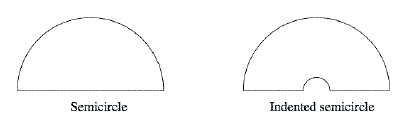
\includegraphics[width=10cm]{semicircle.png}
\end{figure}
Most common ones.

You have use them to solve 
$$\int_0^{\infty}\dfrac{\sin x}{x}dx,\,\,\,\,\int_{-\infty}^{\infty}\dfrac{\cos x}{x^2+a^2}dx,\,\,\,\,\int_{-\infty}^{\infty}\dfrac{x\sin x}{x^2+a^2}dx,\,\,\,\,\int_{-\infty}^{\infty}\dfrac{dx}{1+x^4}$$
$$\int_0^{\infty}\dfrac{x\sin x}{(x^2+4)^2}dx,\,\,\,\,\int_{-\infty}^{\infty}\dfrac{dx}{(1+x^2)^{n+1}}dx,\,\,\,\,\int_{0}^{\infty}\dfrac{1-\cos x}{x^2}dx$$
\end{block}
\end{frame}

\begin{frame}
\begin{block}{Countour 2----Sector}
\begin{figure}[h]
    \centering
    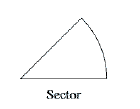
\includegraphics[width=4cm]{sector.png}
\end{figure}
Similar to Semi-circle.

May be useful for integral containing $\sin(x^n)$, $\cos(x^n)$ 

(choose central angle=$\dfrac{\pi}{2n}$) 

You have use it to solve 
$$\int_0^{\infty}\sin^2xdx,\,\,\,\,\int_{0}^{\infty}\cos^2xdx$$
\end{block}
\end{frame}

\begin{frame}
\begin{block}{Countour 3}
\begin{figure}[h]
    \centering
    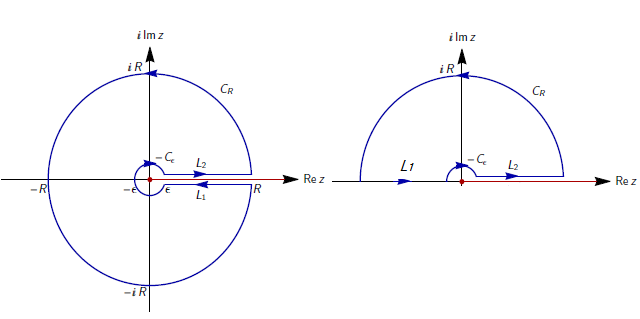
\includegraphics[width=10cm]{branch.png}
\end{figure}

Used for integral containing $\sqrt{x}$, $\ln x$ (For these two countours, the branch we choose is $\mathbb{C}\setminus\mathbb{R}^0_-$, so $\phi\in(0,2\pi)$)

$$\int_0^{\infty}\dfrac{\sqrt{x}}{x^2+a^2}dx,\,\,\,\,\int_{0}^{\infty}\dfrac{\ln x}{x^2+a^2}dx$$
\end{block}
\end{frame}


\begin{frame}
\begin{block}{Residue Calculus for Functions with Branch Points}
Let $P$ and $Q$ be polynomials of degree $m$ and $n$, respectively, where $n\geqslant m+2$. If $Q(x)\neq0$ for $x>0$, if $Q$ has a zero of order at most 1 at the origin and if
$$f(z)=\dfrac{z^{\alpha}P(z)}{Q(z)},\hspace{3mm}0<\alpha<1$$
then
$$\text{p.v.}\int_0^{\infty}\dfrac{x^{\alpha}P(x)}{Q(x)}dx=\dfrac{2\pi i}{1-e^{2\pi \alpha i}}\sum\limits_{j=1}^k\text{res}_{z_j}f$$
\end{block}
This theorem is obtained by using the countour in the left on last slide. Pay attention to the branch. Also pay attention to its requirement. 
\end{frame}

\begin{frame}
\begin{block}{Countour 4}
\begin{figure}[h]
    \centering
    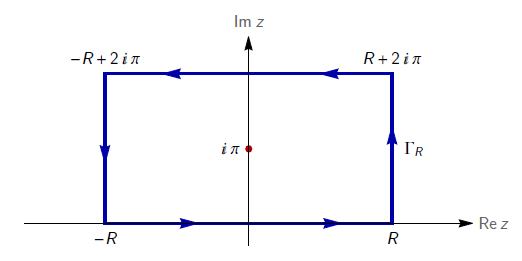
\includegraphics[width=8cm]{rectangle.png}
\end{figure}

$$\int_0^{\infty}\dfrac{e^{ax}}{1+e^x}dx$$
\end{block}
\end{frame}

\begin{frame}
\begin{block}{Jordan's Lemma}
Assume that for some $R_0>0$ the function $g:\mathbb{C}\setminus B_{R_0}(0)\rightarrow\mathbb{C}$ is holomorphic. Let
$$f(z)=e^{iaz}g(z),\hspace{3mm}\text{for some }a>0$$
Let
$$C_R=\lbrace z\in\mathbb{C}:z=R\cdot e^{i\theta},0\leqslant\theta\leqslant\pi\rbrace$$
be a semi-circle segement in the upper half-plane and assume that
$$\sup_{0\leqslant\theta\leqslant\pi}|g(Re^{i\theta})|\xlongrightarrow{R\rightarrow\infty}0$$
Then
$$\lim_{R\rightarrow \infty}\int_{C'_R}f(z)dz=0$$
($C'_R\subset C_R$)
\end{block}
\end{frame}


\begin{frame}
The following theorem is used to prove Cauchy's Theorem.
\begin{block}{Goursat's Theorem}
Let $\Omega\subset\mathbb{C}$ be an open and $f$ \textcolor[rgb]{0,0.6,0.3}{\textit{\textbf{holomorphic}}} on $\Omega$. Let $T\subset\Omega$ be a \textcolor[rgb]{0,0.6,0.3}{\textit{\textbf{triangle}}} whose interior is also contained in $\Omega$. Then
$$\oint_Tf(z)dz=0$$
and therefore, for a \textcolor[rgb]{0,0.6,0.3}{\textit{\textbf{rectangle}}} $R$,
$$\oint_Rf(z)dz=0$$
\end{block}
\end{frame}

\begin{frame}

\begin{block}{Morera's Theorem}
Let $\Omega\subset\mathbb{C}$ be an open, connected set and let $f : \Omega \rightarrow \mathbb{C}$ be continuous. Suppose that 
$$\oint_Tf(z) dz = 0\hspace{3mm} \text{for any triangle \textit{T} wholly contained in }\Omega$$
\begin{enumerate}
\item $f$ has a primitive on $\Omega$
\item ($f$ is holomorphic.) 
\end{enumerate}
\end{block}
For the proof of this theorem, it's similar to the one in below.
\begin{block}{Local Existence of Primitives}
A holomorphic function in an open disc has a primitive in that disc. (P316)
\end{block}
\end{frame}


\begin{frame}
\begin{block}{Proof}
$\forall z\in\Omega$, choose some $z_0$ such that $z\in B_{\delta}(z_0)$ for some $\delta>0$. Then define the function
$$F:B_{\delta}(z_0)\rightarrow\mathbb{C},\hspace{3mm}F(z)=\int_{\mathcal{C}(z_0,z)}f(\zeta)d\zeta$$
where $\mathcal{C}(z_0,z)$ is parametrized by 
$$\gamma:[0,1]\rightarrow\mathbb{C},\hspace{3mm}\gamma(t):=(1-t)z_0+tz$$

Suppose that $z+h\in B_{\delta}(z_0)$ for some $h$. Any integral along the triangle with vertices $z_0,z$ and $z+h$ vanishes, so that
\begin{align*}
F(z+h)-F(z)&=\int_{\mathcal{C}(z,z+h)}f(\zeta)d\zeta=\int_0^1f((1-t)z+t(z+h))\cdot hdt\\
&=h\int_0^1f(z+th)dt
\end{align*}
\end{block}
\end{frame}

\begin{frame}
\begin{block}{Proof (continued)}
Since $f$ is continuous, $f(z+th)=f(z)+\psi(h)$, where $\psi(h)\rightarrow0$ as $h\rightarrow0$, so
$$F(z+h)=F(z)+hf(z)+o(h)$$
So $F'(z)=f(z)$. A holomorphic function is automatically infinitely often differentiable. So $f(z)$ is holomorphic.
\end{block}
\end{frame}


\begin{frame}
\frametitle{Cauchy Integral Formulas}
Suppose $f$ is a holomorphic function in an open set $\Omega\subset\mathbb{C}$. If $D$ is an open disc whose closure is contained in $\Omega$ then
$$f(z)=\dfrac{1}{2\pi i}\oint_C\dfrac{f(\zeta)}{\zeta-z}d\zeta$$
where $C=\partial D$ is the (positively oriented) boundary circle of $D$. (It holds for all toy contours.)
\begin{block}{}
If $f$ is a holomorphic function in an open set $\Omega\subset\mathbb{C}$, then $f$ has infinitely many complex derivatives in $\Omega$. Moreover, if $D$ is an open disc whose closure is contained in $\Omega$,
$$f^{(n)}=\dfrac{n!}{2\pi i}\oint_C\dfrac{f(\zeta)}{(\zeta-z)^{n+1}}$$
where $C=\partial D$ is the (positively oriented) boundary circle of $D$.
\end{block}
\end{frame}

\begin{frame}
\frametitle{Holomorphic Functions are Analytic}
Suppose $f$ is a holomorphic function in an open set $\Omega$. If $D$ is an open disc centered at $z_0$ whose closure is contained in $\Omega$, then $f$ has a power series expansion at $z_0$
$$f(z)=\sum\limits_{n=0}^{\infty}a_n(z-z_0)^n$$
for all $z\in D$ and the coefficients are given by
$$a_n=\dfrac{f^{(n)}(z_0)}{n!},\hspace{3mm}n\in\mathbb{N}$$
\end{frame}


\begin{frame}
\begin{block}{Uniqueness of Holomorphic Functions}
Let $\Omega\subset\mathbb{C}$ be a region and $f,g:\Omega\rightarrow\mathbb{C}$ two holomorphic functions. Suppose that $S\subset\Omega$ has an accumulation point that is contained in $\Omega$ and that
$$f(z)=g(z)\hspace{3mm}\text{for all }z\in S$$
Then $f(z)=g(z)$ for all $z\in\Omega$.
\end{block}
\begin{block}{Analytic Continuation}
Let $M\subset\mathbb{C}$ be a any set and $f:M\rightarrow\mathbb{C}$ any function. Let $\Omega$ be a region with $M\subset\Omega$ and $g:\Omega\rightarrow\mathbb{C}$ a holomorphic function such that $g(z)=f(z)$ for $z\in M$. Then $g$ is called an analytic continuation of $f$ to $\Omega$.
\end{block}
\end{frame}




\end{document}
